% LaTeX file for a 1 page document
\documentclass[oneside, a4paper, 11pt]{memoir}
\usepackage[utf8]{inputenc}
\usepackage[T1]{fontenc}
%\usepackage[ngerman,english]{babel}

\usepackage{amsmath}
\usepackage[squaren,thinspace,thinqspace]{SIunits}
\usepackage[minionint, lf]{MinionPro}
\usepackage[medfamily, sansmath, lf]{MyriadPro}

\usepackage{microtype}
\usepackage{graphicx}
\usepackage[normalem]{ulem}
\usepackage{lipsum}
\usepackage[round]{natbib}
\usepackage{url}
\usepackage{verbments}

%\usepackage{titlesec}
%\titlespacing*{\subsubsection}{0pt}{0.5\baselineskip}{0.3\baselineskip}

% *************** Page layout ***************
% set up recto (right) page layout
%\settypeblocksize{620pt}{400pt}{*}
%\setulmargins{3.5cm}{*}{*}
%\setlrmargins{3cm}{*}{*}
%%\setlrmargins{*}{*}{1.4}
%\setheadfoot{\onelineskip}{2\onelineskip}
%\setheaderspaces{*}{1.5\onelineskip}{*}
%\checkandfixthelayout
%% Make even page margins similar to odd page margins to enable proper
%% single-sided printing (Pg. 25 Memoir documentclass manual)
%\setlength{\evensidemargin}{\oddsidemargin}

\usepackage{geometry}
\geometry{
	a4paper,
	total={210mm,297mm},
	left=35mm,
	right=30mm,
	top=30mm,
	bottom=30mm,
}

\setsecnumdepth{subsection}
\maxsecnumdepth{subsection}

%\pagestyle{ruled}
\nouppercaseheads

\newenvironment{itmz}{
	\begin{itemize}
		\setlength{\itemsep}{0pt}
		\setlength{\parskip}{0pt}
	}{\end{itemize}}

%\fixpdflayout

% *************** Caption font configuration ****************
%\captionstyle[\centering]{\raggedright}
%\captionnamefont{\sffamily\footnotesize\bfseries}
%\captiontitlefont{\sffamily\footnotesize\mathversion{sans}}
%\renewcommand{\parttitlefont}{\Huge\sffamily\bfseries}

%\setsecheadstyle{\sffamily\Large\bfseries\hrule\vspace{2pt}}
%\setsecheadstyle{\sffamily\bfseries\Large}
%\setsubsecheadstyle{\sffamily\bfseries\large}
%\setsubsubsecheadstyle{\sffamily\bfseries\slshape\large}

\title{Fault tolerance mechanisms on SpiNNaker}

\begin{document}
\maketitle

%\begin{abstract}
%The reconstruction conjecture states that the multiset of unlabeled
%vertex-deleted subgraphs of a graph determines the graph, provided it
%has at least 3 vertices.  A version of the problem was first stated
%by Stanis\l aw Ulam.  In this paper, we show that the conjecture can
%be proved by elementary methods.  It is only necessary to integrate
%the Lenkle potential of the Broglington manifold over the quantum
%supervacillatory measure in order to reduce the set of possible
%counterexamples to a small number (less than a trillion).  A simple
%computer program that implements Pipletti's classification theorem
%for torsion-free Aramaic groups with simplectic socles can then
%finish the remaining cases.
%\end{abstract}

%\mainmatter
%\chapter{Fault tolerance mechanisms}

\chapter{Introduction}
The three fault-tolerant mechanisms that will be dealt with in this report are:
\begin{itemize}
\item Dumped packet re-insertion
\item Process migration -- currently implemented on the heat demo, where a core fault is simulated by intentionally reset a core. Currently if core 1 on core (0,0) is reset or disabled no communication is possible with the host PC.
\item CRC error detection/correction of SDRAM blocks
\end{itemize}
	
\section{Useful books and links}
\begin{itemize}
\item Sorin, Fault tolerant computer architecture. Ch. 3 Error recovery (FER and BER).
\item Avresky, Fault-tolerant Parallel and Distributed Systems. Part II.4 Fault-tolerant distributed systems. Part IV (all).
\item Abd-El-Barr, Design and analysis of reliable and fault-tolerant computer systems. Seems to treat fault tolerance of networks in depth. Chps. 1, 2, 3, 4, Ch. 13 Algorithm-Based Fault tolerance.
\item Goloubeva, Software-Implemented Hardware Fault tolerance. Ch1. Background and Ch. 4 Achieving fault tolerance.
\item Checkpointing and recovery, \url{http://srel.ee.duke.edu/sw_ft/node9.html}
\end{itemize}

\section{SpiNNaker architecture}
\begin{figure}[htbp]
	\centering
	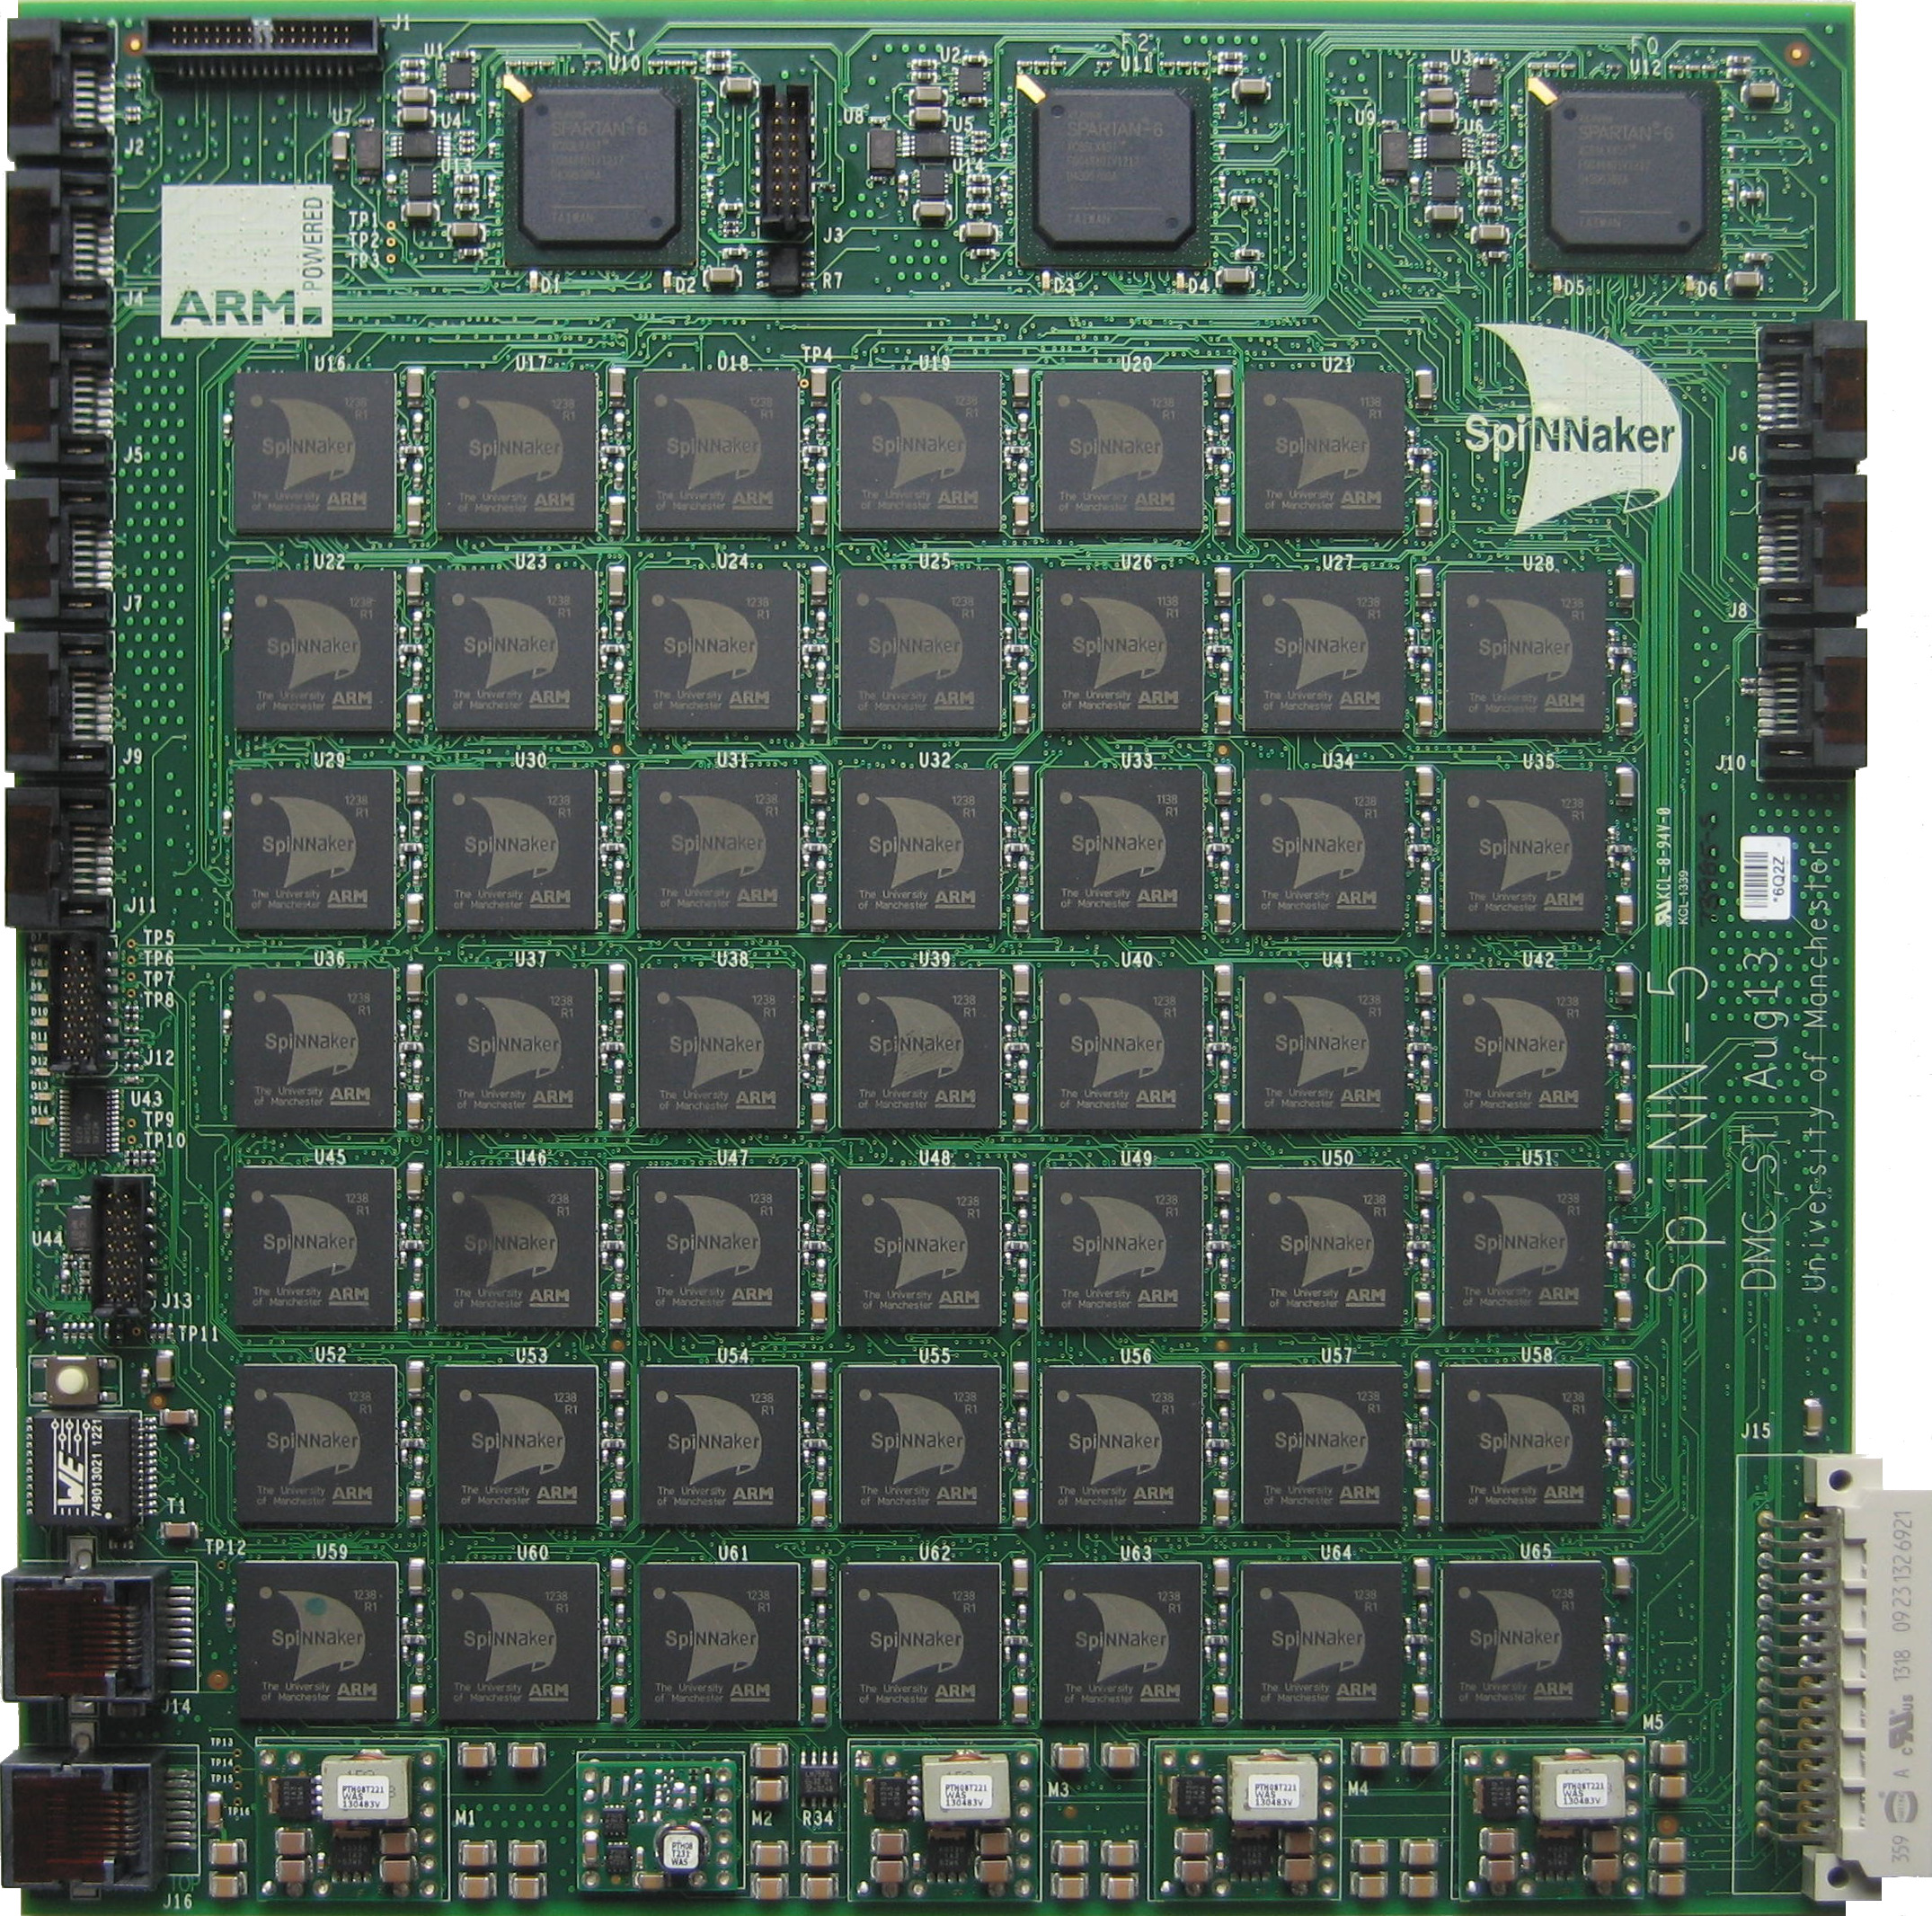
\includegraphics[width=0.6\linewidth]{images/spin5.jpg}
	\caption{48-chip Spin5 board}
\end{figure}

\begin{figure}[htbp]
	\centering
	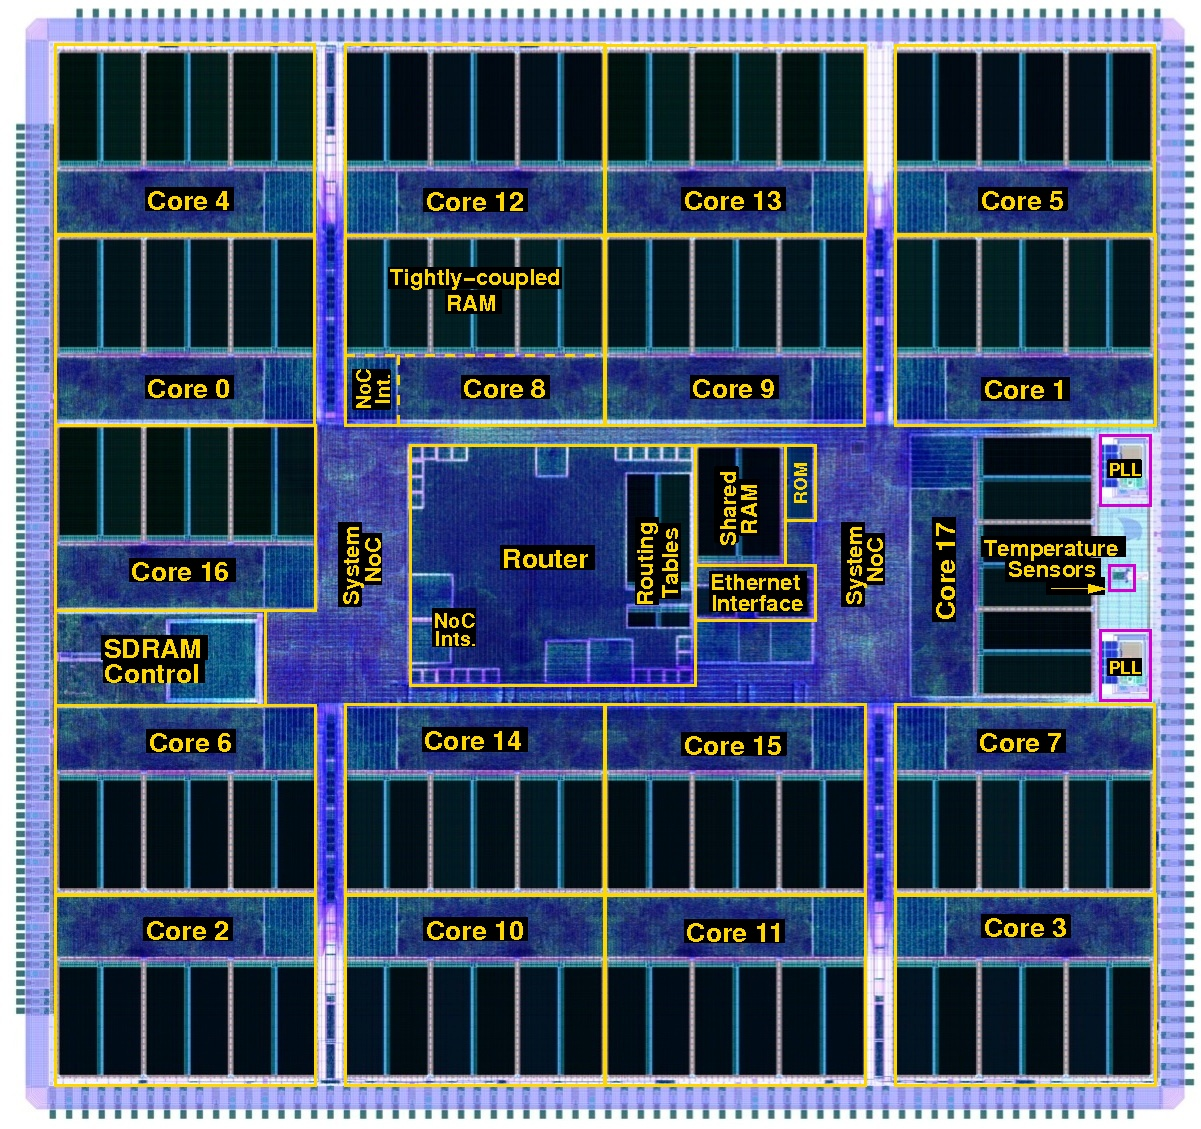
\includegraphics[width=0.5\linewidth]{images/spin2_labelled.jpg}
	\caption{Labelled SpiNNaker die}
\end{figure}

\begin{figure}[htbp]
	\centering
	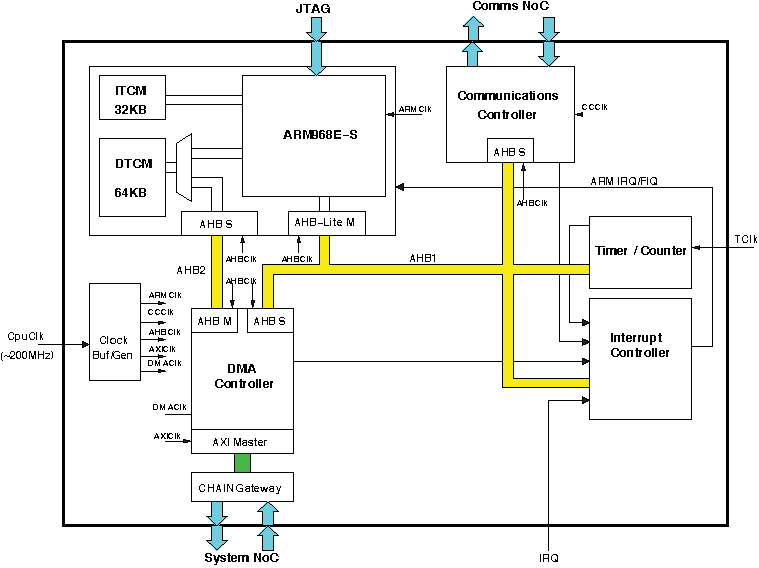
\includegraphics[width=0.8\linewidth]{images/arm968_subsystem.pdf}
	\caption{ARM 968 subsystem}
\end{figure}

\begin{figure}[htbp]
	\centering
	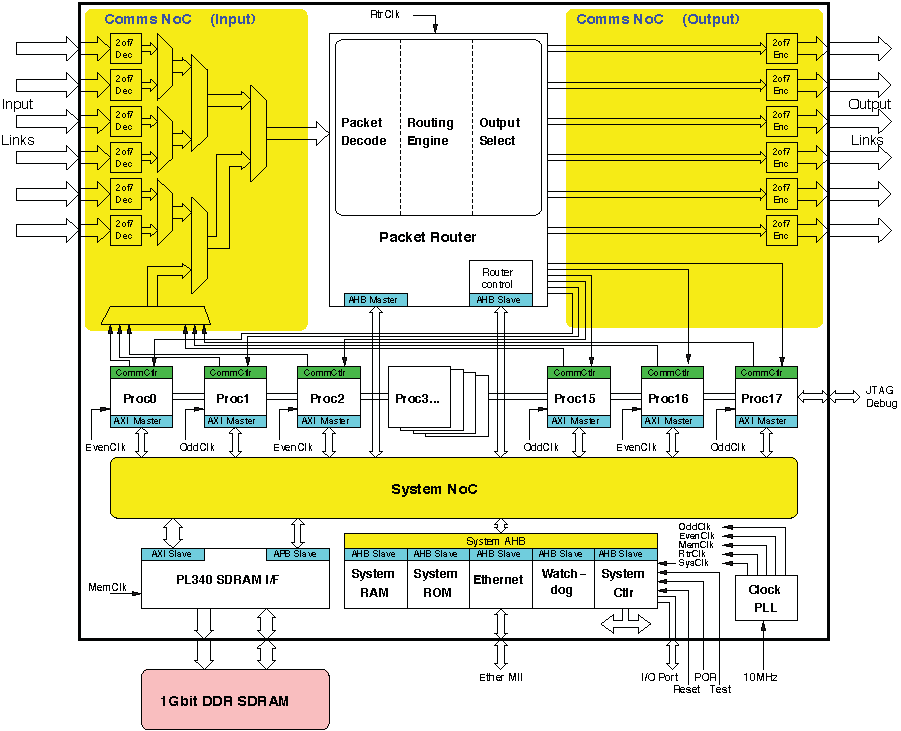
\includegraphics[width=0.8\linewidth]{images/spinnaker_architecture.pdf}
	\caption{SpiNNaker architecture}	
\end{figure}

\begin{figure}[htbp]
	\centering
	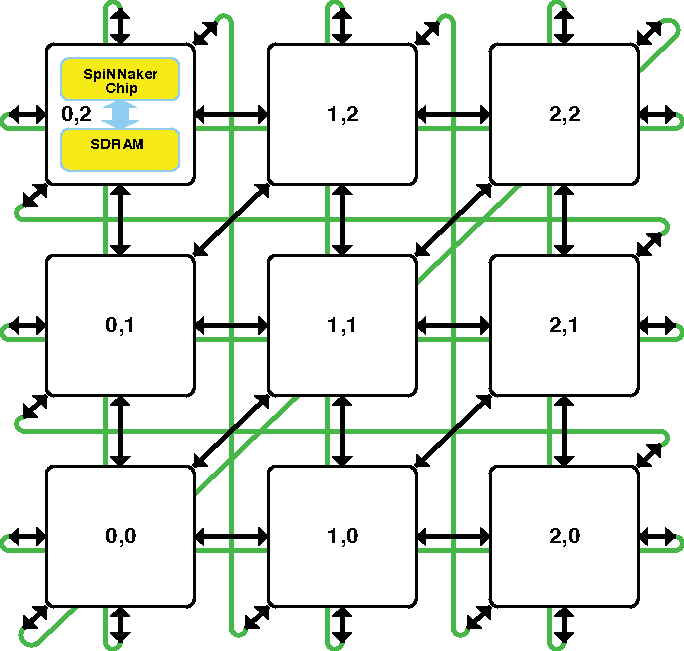
\includegraphics[width=0.4\linewidth]{images/system_architecture.pdf}
	\caption{System architecture}	
\end{figure}

\begin{figure}[htbp]
	\centering
	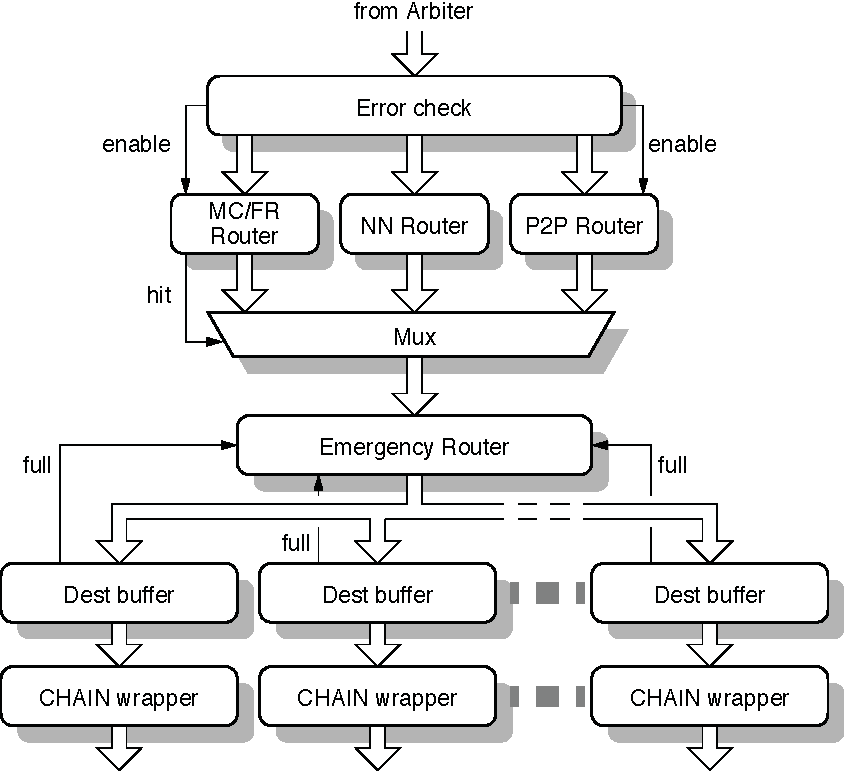
\includegraphics[width=0.6\linewidth]{images/router_organization.pdf}
	\caption{Router organization}	
\end{figure}

\chapter{Dumped packet reinsertion}

\chapter{Process migration}
\begin{verbatim}
To test out the heat_demo_ft functionality, start the heat_demo_ft.aplx
by running (from ybug) @ heat_demo_ft_1board.ybug

Then start resetting cores one-by-one by writing directly to the system
controller register (0xe2000000:r1 = 0xe2000004)
command: sw 0xe2000004 0x5ec00002

Note: The core you reset happens to be the leadAp, the application will
crash.
\end{verbatim}

\chapter{CRC error correction}

\section{Wikipedia description of discrete logarithm}
In mathematics, a discrete logarithm is an integer k solving the equation $b^k = g$, where $b$ and $g$ are elements of a finite group. Discrete logarithms are thus the finite-group-theoretic analogue of ordinary logarithms, which solve the same equation for real numbers $b$ and $g$, where $b$ is the base of the logarithm and $g$ is the value whose logarithm is being taken.

Computing discrete logarithms is believed to be difficult. No efficient general method for computing discrete logarithms on conventional computers is known, and several important algorithms in public-key cryptography base their security on the assumption that the discrete logarithm problem has no efficient solution.

\subsection{Example}
Discrete logarithms are perhaps simplest to understand in the group $(\mathbf{Z}_p)^\times$. This is the group of multiplication modulo the prime $p$. Its elements are congruence classes modulo $p$, and the group product of two elements may be obtained by ordinary integer multiplication of the elements followed by reduction modulo $p$.

The $k$th power of one of the numbers in this group may be computed by finding its $k$th power as an integer and then finding the remainder after division by $p$. When the numbers involved are large, it is more efficient to reduce modulo $p$ multiple times during the computation. Regardless of the specific algorithm used, this operation is called modular exponentiation. For example, consider $(\mathbf{Z}_{17})^\times$. To compute 34 in this group, compute $34 = 81$, and then divide 81 by 17, obtaining a remainder of 13. Thus $34 = 13$ in the group $(\mathbf{Z}_{17})^\times$.

The discrete logarithm is just the inverse operation. For example, consider the equation $3k \equiv 13$ (mod 17) for $k$. From the example above, one solution is $k = 4$, but it is not the only solution. Since $316 \equiv 1$ (mod 17)---as follows from Fermat's little theorem---it also follows that if $n$ is an integer then $34+16n \equiv 34 \times (316)n \equiv 13 \times 1^n \equiv 13$ (mod 17). Hence the equation has infinitely many solutions of the form $4 + 16n$. Moreover, since 16 is the smallest positive integer $m$ satisfying $3m \equiv 1$ (mod 17), i.e. 16 is the order of 3 in $(\mathbf{Z}_{17})^\times$, these are the only solutions. Equivalently, the set of all possible solutions can be expressed by the constraint that $k \equiv 4$ (mod 16).

\subsection{Algorithms}
No efficient classical algorithm for computing general discrete logarithms logb g is known. The naive algorithm is to raise b to higher and higher powers k until the desired g is found; this is sometimes called trial multiplication. This algorithm requires running time linear in the size of the group G and thus exponential in the number of digits in the size of the group. There exists an efficient quantum algorithm due to Peter Shor.[1]

More sophisticated algorithms exist, usually inspired by similar algorithms for integer factorization. These algorithms run faster than the naive algorithm, some of them linear in the square root of the size of the group, and thus exponential in half the number of digits in the size of the group. However none of them runs in polynomial time (in the number of digits in the size of the group).

%\begin{itemize}
%\setlength{\itemsep}{0pt}
%\item Baby-step giant-step
%\item Function field sieve
%\item Index calculus algorithm
%\item Number field sieve
%\item Pohlig–Hellman algorithm
%\item Pollard's rho algorithm for logarithms
%\item Pollard's kangaroo algorithm (aka Pollard's lambda algorithm)
%\end{itemize}

\subsection{Comparison to integer factorization}
While computing discrete logarithms and factoring integers are distinct problems, they share some properties:

\begin{itemize}
	\setlength{\itemsep}{-2pt}
	\item both problems are difficult (no efficient algorithms are known for non-quantum computers),
	\item for both problems efficient algorithms on quantum computers are known,
	\item algorithms from one problem are often adapted to the other, and
	\item the difficulty of both problems has been used to construct various cryptographic systems.
\end{itemize}

\section{Abstract}
Error-control codes provide a mechanism to increase the reliability of digital data being processed, transmitted, or stored under noisy conditions. Cyclic codes constitute an important class of error-control code, offering powerful error detection and correction capabilities. They can easily be generated and verified in hardware, which makes them particularly well suited to the practical use as error detecting codes.

A cyclic code is based on a generator polynomial which determines its properties including the specific error detection strength. The optimal choice of polynomial depends on many factors that may be influenced by the underlying application. It is therefore advantageous to employ programmable cyclic code hardware that allows a flexible choice of polynomial to be applied to different requirements. A novel method is presented in this thesis to realise programmable cyclic code circuits that are fast, energy-efficient and minimise implementation resources.

It can be shown that the correction of a single-bit error on the basis of a cyclic code is equivalent to the solution of an instance of the discrete logarithm problem. A new approach is proposed for computing discrete logarithms; this leads to a generic deterministic algorithm for analysed group orders that equal Mersenne numbers with an exponent of a power of two. The algorithm exhibits a worst-case runtime in the order of the square root of the group order and constant space requirements.

This thesis establishes new relationships for finite fields that are represented as the polynomial ring over the binary field modulo a primitive polynomial. With a subset of these properties, a novel approach is developed for the solution of the discrete logarithm in the multiplicative groups of these fields. This leads to a deterministic algorithm for small group orders that has linear space and linearithmic time requirements in the degree of defining polynomial, enabling an efficient correction of single-bit errors based on the corresponding cyclic codes.

\section{Introduction}
The preservation of digital data integrity is of major concern for computer, communication, and storage systems. In all these applications digital data is susceptible to unintentional modification which may arise from electrical or magnetic disturbance, component failure, or the result of system design error. Depending on the specific application, data failures may result in severe consequences and thus their potential occurrence needs to be considered carefully in the underlying design of the system.

Data reliability can be enhanced through the employment of error-control codes,which provide mechanisms for the detection and correction of errors. These codes enrich the data with redundancy by forming code words, which initially can be used to detect inconsistencies in the received data. If the affected data can be retransmitted or recalculated, one simple error correction scheme is the Automatic Repeat Query (ARQ), where the receiver simply requests a retransmission once it detects data inconsistencies. However, where retransmission or recalculation is not feasible, being too slow or uneconomic, Forward Error Correction (FEC) techniques can correct errors on the basis of the corrupted received data and its inherent redundancy.

Cyclic codes form an important class of error-control code offering powerful error detection and correction capabilities. At the same time, their algebraic properties permit the use of simplified processing procedures when compared to non-cyclic codes. For instance, the encoding of data into cyclic code words can easily be achieved in hardware using a simple linear feedback shift register. Likewise, the same circuit can be used to validate code words, and thus detect errors. For these reasons, cyclic codes have been widely adopted as error-detecting codes and commonly deployed in combination with ARQ schemes. This thesis concentrates on cyclic codes with symbols from the binary field.

If error correction is desired, the most basic case concerns the localisation of a single erroneous bit. It can be shown that for cyclic codes this problem is equivalent to the computation of the discrete logarithm in finite cyclic groups, for which it is

widely believed that for the general case no efficient classical algorithm is devisable. This is one reason why the discrete logarithm forms the basis for many cryptographic applications such as the Diffie-Hellman-Merkle key exchange. However, it has not been proven that the computation of the discrete logarithm is hard for all groups of practical interest.

Cyclic codes are characterised by an underlying generator polynomial. Different generator polynomials exhibit different capabilities in regard to the detection and correction of errors. Certain polynomials, for example,may be particularly well suited to the practical realisation of the error correction process. The selection of polynomial is also dependent on the length of the data that is to be protected and the anticipated error patterns. In systems where diverse applications may favour different cyclic codes, and where the requirements may change over time or be unknown at the design stage, it may be advantageous to provide full flexibility in regard to the usable cyclic code generator polynomials. Efficient cyclic code processing relies on dedicated cyclic code hardware circuits, which may be programmable if the underlying generator polynomial is adaptable. Such a programmable circuit has been created for the SpiNNaker project, a massively parallel spiking neural network simulator.

\section{Objectives}
Cyclic codes comprise a powerful class of error-control code; they have gained wide popularity in the field of error detection owing to their efficient hardware implementations and simultaneous effective error detection. Programmable cyclic code circuits have the benefit of flexible adaptation of the underlying cyclic code to meet the requirements of a specific application. One goal of this research is to provide a method for the efficient realisation of parallel programmable cyclic code circuits, in hardware, to make them appealing for a wider range of applications.

The current predominating drawback of cyclic codes is the lack of efficient error correction techniques for them. To perform the correction of a single-bit error an instance of the generalised discrete logarithm problem needs to be solved. It is an additional goal of this research to explore new methods in the quest for an efficient mechanism for computing discrete logarithms in relevant finite cyclic groups and, therefore, facilitate the efficient recovery from single-bit errors through cyclic codes.

\section{Contribution}
The contributions of this thesis are summarised as follows:

\begin{itemize}
\item A new scheme is proposed enabling the efficient calculation of the state transition and control matrix for the parallel operation of a cyclic code circuit in hardware. This circuit is used both for the data encoding step and the decoder error detection phase. With the incorporation of a programmable transition and control matrix, this adaptable circuit can be configured to use different cyclic codes. This added flexibility is a valuable enhancement, as the error detection and error correction performance of a particular cyclic code depends on parameters including the length of the data that is to be protected and the anticipated error patterns of an application. A simulation of the novel programmable cyclic code circuit produced shows significant improvements in terms of speed, area and energy efficiency when compared with previously published designs. The design of the new circuit has been published [GF11].
\item A new approach is proposed for the computation of discrete logarithms; this leads to a generic deterministic algorithm for analysed group orders that equal a Mersenne number where the exponent is a power of two. It is shown that, for these groups, the worst-case running time is proportional to the square root of the group order, while the space requirements are constant. The scheme is further improved for particular cases where the discrete logarithm values occur with different probabilities, leading to reduced average and worst-case execution times. Furthermore, properties are derived that apply to the sequences that are used by the algorithm.
\item A set of new relationships is developed for the field elements of the ring of polynomials over the binary field modulo a primitive polynomial. Based on a subset of these properties, a novel approach is proposed for the computation of discrete logarithms in the cyclic multiplicative group of the finite field. For at least all primitive polynomials up to degree 12 and the first evaluated primitive polynomials of degree 13 and 14, a deterministic algorithm with linear space and linearithmic time requirements in the degree of the polynomial results.
\end{itemize}

\section{Thesis overview}
\subsection{Chapter 4}
This chapter presents an overview of the SpiNNaker project which targets the large-scale simulation of spiking neural networks. The SpiNNaker architecture facilitates a massively-parallel supercomputer with a million processors, which supports these neural simulations. The issue of anticipated memory faults in a SpiNNaker system of this scale is highlighted, and the usage of cyclic codes as a layer of protection against many of these errors is explained.

\subsection{Chapter 5}
In this chapter, the equations for a parallel realisation of a cyclic code circuit are derived. It is then shown how a programmable version of such a circuit can be created which can be configured to use different generator polynomials. Furthermore, a new scheme is presented that allows the efficient computation of the state transition and control matrix necessary for the circuit. With this scheme a novel programmable parallel cyclic code circuit is proposed that is then compared to previous work. This chapter is based on a journal publication [GF11].

\subsection{Chapter 6}
This chapter describes a new generic approach for the computation of the discrete logarithm. Based on this approach an algorithm is presented for group sizes that equal a Mersenne number with an exponent of a power of two. It is shown how the scheme can be improved if the discrete logarithm values occur with unequal probabilities. Properties are derived for the sequences that are used by the algorithm and finally, the proposed scheme is compared with an established method for the evaluation of discrete logarithms.

\subsection{Chapter 7}
In this chapter, a new set of properties is derived for the elements of a finite field with binary characteristic, where the field is represented as a polynomial ring over the binary field modulo a primitive polynomial. For the multiplicative group of the finite field, a novel approach is presented to compute discrete logarithms based on a subset of the newly established field properties. Performance results are reported for the resulting algorithm for evaluated small group sizes.


\newpage
\section{Excerpts from Chapter 4 -- SpiNNaker}
\subsection{Memory}
The large SpiNNaker system in its envisaged configuration of 57,600 nodes will incorporate in the order of 7 TiB of SDRAM. With such an immense amount of memory, the effect of data bit errors is significant during the operation of the machine.

Memory bit errors are subdivided into two different classes: hard and soft errors [ZL79; Zie96; Zie+96].A hard error is characterised by a permanent hardware fault in a memory cell that will result in a consistent reliability issue. For instance, it may be the case that a memory cell will always provide one particular bit value during readout, no matter what value has been written to it. Soft errors are transient faults that occur randomly and may, for example, be induced through cosmic rays or the decay of radioactive atoms in the memory packaging materials. Also, a soft error may arise either directly in the memory, or along the data path during the memory read or write phase.

Recently, a large-scale study has been conducted to investigate statistics for error rates in Dynamic Random Access Memory (DRAM) in production systems [SPW09]. It suggests that the average error rate ranges from 25,000 to 75,000 FIT (failures in time per billion hours of operation) per Mibit, however a distinction between hard and soft errors is not made. If these numbers are applied to the SpiNNaker system of 57,600 nodes, 25 to 74 bit errors on average can be expected to occur within the SDRAM per minute, roughly approximated as one bit error per second.

It may be the case that the number of expected bit errors in the SpiNNaker system will not have a significant impact on particular applications such as neural network simulations. However, it is not known to what extent neural network simulations can compensate for memory faults, and other potential applications may not tolerate bit errors at all, so appropriate measures need to be taken to deal with them in the SpiNNaker system. For this reason error-control codes are employed within SpiNNaker to provide a layer of protection against memory faults.

\subsection{CRC unit}
The DMA controller of each processing subsystem has been equipped with a CRC unit that allows the generation and verification of error-control codes. The circuit primarily supports cyclic codes as they offer powerful error detection and correction capabilities and as they are, at the same time, easily implementable in hardware [LC83]. If, for instance, a processor initiates a DMA transfer to copy a data block from the local memory to the SDRAM, the CRC unit can be instructed to calculate (transparently and in parallel) the redundancy part for a cyclic code and, automatically, append this to the SDRAM data block. The CRC unit can be used to calculate the error syndrome for a data block retrieved from memory and signal the corresponding processing core if an integrity issue arose. The program that is executed on the processing core has to decide what action is to be taken in the event of a detected data inconsistency. A simple retransmission of the data block could correct the error if it occurred along the data path during the readout phase, however even this may not be fast enough for the `real-time' operation of a SpiNNaker neural simulation. Therefore it is necessary to consider appropriate error correction procedures in software, to recover from memory faults based on the obtained error syndrome, including when they are uncorrectable. These can range from a simple disregard of the error, through a localisation and correction of the error, to a shutdown of the relevant SpiNNaker system components for replacement if hard errors are involved.

In the choice of employed cyclic code, many factors need to be taken into account for the selection of the generator polynomial as outlined in Subsection 2.3.4. For instance, certain undiscovered subclasses of cyclic codes may allow the realisation of very efficient error correction procedures in software, or data blocks of different lengths may be stored in the SDRAM so that a polynomial offering best combined error protection for all of the block lengths should be selected. To offer maximal flexibility within SpiNNaker, a programmable CRC circuit has been incorporated that permits switching the generator polynomial to any of degree 32 or lower whenever required. A direct advantage is that the polynomial is adaptable to the length of the data block that is to be protected, which means that the best choice of offered error protection can be made. Another feature of the CRC circuit is that several cyclic codes of a smaller degree can be generated based on different bits of the data stream. For example, for each half-word of the data stream, a cyclic code based on a generator polynomial of degree 16 can be computed.

The width of the data bus that traverses the DMA controller in SpiNNaker is 32 bits, and the CRC unit has been designed to process this number of bits in parallel to avoid being a bottleneck to DMA data transfers. To configure the unit for the usage of a cyclic code or any other supported error-control code, one Kibit of configuration data needs to be supplied by the corresponding processing core to the appropriate registers inside the unit. Since the data bus is used to provide this configuration data, the transfer takes place as a series of 32 bit words. The registers are realised as latches to reduce the hardware demand, as each SpiNNaker chip accommodates one CRC unit for each of the 18 DMA controllers (one per processor subsystem). A detailed description of the SpiNNaker CRC circuit together with its derivation and capabilities can be found in the next chapter.

\subsection{Conclusion}
The SpiNNaker architecture has been created to support large-scale simulations of spiking neural networks in biological real-time. It has been dimensioned to scale up to machines consisting of a million processors with SDRAM totalling about 7 TiB. With such a vast amount of memory, it is estimated that, on average, about 1 bit error per second will occur.

To improve the reliability of memory transfers, SpiNNaker employs cyclic codes for error control due to the efficient realisation of the code generation and verification circuit. Once inconsistencies are detected for a block of data, software procedures may be triggered to attempt an error recovery. The correction of a single-bit error on the basis of a cyclic code, essentially requires the computation of the discrete logarithm in relevant groups as described in Chapter 2. However, no efficient algorithm is known for the computation of this type of discrete logarithm as discussed in Chapter 3. Two new solutions for the computation of the discrete logarithm in certain groups are proposed in Chapter 6 and Chapter 7.

The optimal choice of cyclic code to employ is influenced by many factors including the length of the data that is to be protected and the desired error control capabilities. Therefore, programmable cyclic code circuits are employed within SpiNNaker to maximise flexibility in the choice of cyclic code for different scenarios. A novel method for the generation of efficient programmable cyclic code circuits is proposed in Chapter 5.

\newpage
\section{Ecerpts from Chapter 5 -- Programmable CRC hardware}
Cyclic codes constitute a powerful class of error-control code as set out in Section 2.3. They offer effective error detection and can easily be realised in hardware, which makes them a popular choice for many applications that require the detection of errors, including Ethernet [TW11]. In the context of pure error detection, a cyclic code is often referred to as a Cyclic Redundancy Checksum (CRC) and the popularity of cyclic codes has led to a number of different software and hardware implementations [LC83; RG88].Speed requirements usually make software schemes impractical and dedicated hardware is needed. The generic hardware approach uses an inexpensive Linear Feedback Shift Register (LFSR), which assumes serial data input. In the presence of wide data buses, the serial computation has been extended to parallel versions that process whole data words based on derived equations and on cascading the LFSR [Spr01]. Various optimisation techniques have been developed that target resource reduction [Bra+96] and speed increase [Der01; CP06; KRM08; KRM09].

A wide range of factors influence the selection of an appropriate CRC generator polynomial for a particular application as outlined in Subsection 2.3.4. This range includes the error detection and correction capabilities of a generator polynomial, which depend on the length of the data that is to be protected. For instance, in scenarios where data blocks of different length are used, or where the final requirements of the generator polynomial are not known at the time of the hardware implementation, it is beneficial to employ programmable CRC circuits that can be configured to different generator polynomials.

This applies precisely to the SpiNNaker project, whose target is to provide a research platform for the simulation of arbitrary spiking neural networks as described in Chapter 4. The planned large SpiNNaker system will incorporate a substantial amount of SDRAM to hold relevant data for the neural network simulations; in this context, CRCs are used to reduce the effect of data errors arising in the memory. Since the length of the data blocks may vary between different neural network simulations, for instance, it has been decided to incorporate programmable CRC circuits into the SpiNNaker system to offer maximal flexibility.

With the design of a circuit, there is usually a tradeoff between speed and area. In this particular scenario, there are two dimensions to the speed of a programmable CRC circuit: the time necessary to process a data word, and the time required to reconfigure to a new polynomial. This chapter directly extends the parallel CRC circuit by Campobello et al. [CPR03] based on state space representation in several ways. On the one hand, restrictions between the width of the data processed in parallel and the order of the polynomial are lifted. On the other hand, a novel scheme is presented allowing the inexpensive computation of the CRC transition and control matrix in hardware. This leads to a programmable parallel CRC implementation that offers an improved balance between area and both dimensions of speed.

\newpage
\section{Excerpts from Chapter 8 Conclucion -- Cyclic codes}
Cyclic codes have gained wide popularity as error-detecting codes due to their inherent algebraic properties that permit easy implementation and effective detection of errors. This thesis supports the position of cyclic codes as a powerful class of error-control code whose properties extend beyond simple error detection. The thesis demonstrates contributions in the generation of efficient, programmable, parallel cyclic code circuits, and in the potential of cyclic codes for efficient error correction. These contributions are described in more detail, together with highlighting possible areas for future exploration within this concluding chapter.

\subsection{Programmable CRC}
A cyclic code is characterised through its generator polynomial which influences the specific error detection and correction capabilities of the code, depending on the length of the data that is to be protected, as outlined in Chapter 2. In addition, different applications may run on the same system with completely different cyclic code requirements, as in the case of SpiNNaker which is described in Chapter 4. It was shown how cyclic code circuits can overcome the limitations of a single generator polynomial by allowing the circuit to be flexibly programmed with any polynomial within the design constraints. In Chapter 5 a new method for computing the transition and control matrix of a parallel cyclic code circuit was presented. This method allows the efficient realisation of programmable parallel circuits that operate at high speeds, reconfigure rapidly to new polynomials, require few implementation resources, and are energy-efficient when compared with alternative schemes.

\subsection{Future work in Programmable CRC}
With an efficient programmable cyclic code circuit that can reconfigure rapidly to new generator polynomials, it is feasible to change the polynomial after each processed word of a data stream. The calculation of the next polynomial can be made dependent on factors including the current input data word and the current state of the circuit, i.e. the calculated redundancy and the polynomial. It would be interesting to investigate if a polynomial adjustment algorithm can be devised that has advantages over fixed cyclic code generator polynomials, from both error detection and correction points of view.

\subsection{Error Correction}
The correction of a single-bit error on the basis of a cyclic code requires the computa-tion of the discrete logarithm in finite cyclic groups, represented as the polynomial ring over the binary field modulo the cyclic code generator polynomial, as outlined in Chapter 2. No efficient algorithm is known for the evaluation of the discrete logarithm in these groups and, moreover, it is also widely believed that no such algorithm can be devised as described in Chapter 3. Nonetheless, this work focused on the exploration of new algorithms in the quest for an efficient calculation of discrete logarithms in relevant groups.

A new approach was developed for calculating discrete logarithms in Chapter 6. For groups that have an order equal to a Mersenne number with an exponent of a power of two, a deterministic generic algorithm was devised based on size differences of cyclotomic cosets. The algorithm requires only constant space and exhibits a worst-case asymptotic running time of the square root of the group order. It was shown that the average- and worst-case running times of the algorithm can be improved for certain cases where the discrete logarithm values occur with unequal probabilities. Furthermore, properties were developed or highlighted for relevant sequences that are considered by the algorithm.

For finite fields with binary characteristic, represented as the polynomial ring over the binary field modulo a primitive polynomial, new properties were developed in Chapter 7. On the basis of a subset of these properties, a novel approach was proposed for computing discrete logarithms in the cyclic multiplicative groups of these fields. It resulted in a deterministic algorithm with linear space and linearithmic time requirements in the degree of the defining polynomial, for at least all polynomials up to degree 12 and the first polynomials of degree 13 and 14. The algorithm requires a set of parameters in the order of the polynomial degree, where the parameter search space grows exponentially in the polynomial degree. For this reason partial results on the running time for single polynomials of higher degrees up to 32 were provided.

\subsubsection{Future work in programmable CRC}
\begin{itemize}
\item The research conducted on discrete logarithm algorithms generated a number of open questions that present potential future research opportunities:

\item Under the assumption of the existence of an efficient algorithm for the compu-tation of the discrete logarithm in finite cyclic groups represented in the ring of polynomials modulo a polynomial, the efficient correction of single-bit errors based on cyclic code is feasible. It needs to be investigated further to determine to what extent this assumption would also enable the efficient correction of multi-bit errors.

\item For the proposed algorithm for discrete logarithms for group orders that equal Mersenne numbers with an exponent of a power of two, it may be possible to use the developed sequence properties to improve the algorithm. It may also be the case that new properties can be found that will enable a speed-up of the algorithm. In particular, it needs to be investigated if the proposed algorithm reduces the initial discrete logarithm problem into smaller subgroups, similar to the Silver-Pohlig-Hellman algorithm, as this permits alternative algorithms to be employed in those subgroups.

\item The proposed generic algorithm for discrete logarithms was tailored to group orders of special Mersenne numbers. It remains an open question as to whether the algorithm can be generalised to all group orders and what the resulting execution overheads would be.

\item An algorithm, efficient in time and space, was proposed for the computation of discrete logarithms in the multiplicative groups of small finite fields represented in the polynomial ring over the binary field modulo a primitive polynomial. It was shown that the algorithm is applicable at least to all defining polynomials up to degree 12, and the first polynomials of degree 13 and 14. For single polynomials of degree 15 to 32, it is known that a mapping configuration exists that allows the algorithm to terminate under all conditions, however it is unclear if one exists that also results in an efficient worst-case execution time. It would be interesting to investigate if, for all polynomials with a degree exceeding 12, loop-free mapping configurations exist, and also what would be the best asymptotic worst-case runtime behaviour of the algorithm. A related open question concerns the best achievable average asymptotic runtime of the algorithm.

\item The determination of the overall best mapping configuration for a specific polynomial and optimisation goal was achieved through a brute force attack which is impractical for polynomials of higher degree due to the exponential search space. It may be the case that an efficient method can be devised that allows the computation of the mapping configuration for at least the best worst-or average-case; such a method may also assist in the analysis of the asymptotic runtime behaviours. Alternatively, it may be possible to develop good heuristics to reduce the search space and employ evolutionary algorithms to find a close approximation for the optimal set of values.

\item A number of conjectures were established that need analysis to determine if they can be proven. Proofs for the conjectures concerning the L transformation in particular could lead to further insights into the efficient computation of discrete logarithms in the relevant groups.

\item The proposed algorithm to compute discrete logarithms in multiplicative groups of small finite fields, represented in the polynomial ring over the binary field modulo a primitive polynomial, might also be easily applicable to defining polynomials that are not primitive, but irreducible. If the defining polynomial is reducible, then it induces only a cyclic group, for which the algorithm might also be easily employed. Moreover, it should be investigated if the algorithm can be adapted to finite fields with a characteristic other than two.

\item It was conjectured that, for a defining primitive polynomial of degree m and a parity level l with *** linear transformations of the form T x exist such that each odd parity block of size one on level l is mapped by one of the transformations onto an even parity block element on the same level. It would be interesting to investigate whether, for every level l, a set of these 2l-1 transformations exists, such that the transformations can easily be computed from each other. In particular, it is an open question if the displacement r between the two transformations L2a and L2b for level two can easily be determined, such that L2a = Tr L2b.

\item It is currently unknown if a simple correlation exists between the displacements of equally-sized blocks on a certain parity level. If the displacements can easily be computed, alignments of different parity vector spaces can simply be obtained and therefore also transformations such as E0 and E1.
\end{itemize}

\section{Summary}
The work presented in this thesis provides successful solutions for the addressed research objectives:

\subsection{Efficient Programmable CRC Circuits}

A novel method was proposed for the efficient realisation of programmable parallel cyclic code circuits. The resulting circuits can rapidly be configured with a generator polynomial, exhibit fast operating speeds, have low resource requirements, and are energy-efficient at the same time when compared to alternative solutions.

\subsection{Algorithms for Computing Discrete Logarithms}

Two new approaches were developed for computing discrete logarithms to facilitate the correction of single-bit errors based on cyclic codes.

The first approach is generic in nature leading to a deterministic algorithm for group orders that equal a Mersenne number with an exponent of a power of two; this algorithm has constant space requirements and runs in the worst case in the order of the square root of the group order. It was shown how the algorithm can be improved if the discrete logarithm values occur with unequal probabilities and that certain properties hold for the associated sequences.

The second approach for the computation of discrete logarithms is based on a subset of newly developed properties for finite fields of binary characteristic represented as the polynomial ring over the binary field modulo a primitive polynomial. For evaluated small fields, a deterministic efficient algorithm with linear space and linearithmic time requirements in the degree of the defining polynomial was devised.

\chapter{SpiNNaker Fault tolerance info from datasheet}
\section{ARM 968 (4.3)}
\subsection*{Fault insertion}
\begin{itmz}
\item ARM9TDMI can be disabled.
\item Software can corrupt I-RAM and D-RAM to model soft errors.
\end{itmz}
\subsection*{Fault detection}
\begin{itmz}
\item Self-test routines, run at start-up and during normal operation, can detect faults.
\item A chip-wide watchdog timer catches runaway software.
\end{itmz}
\subsection*{Fault isolation}
\begin{itmz}
\item Defective locations in the I-RAM and D-RAM can be mapped out of use by software.
\item The ARM968 unit can be disabled from the System Controller.
\end{itmz}
\subsection*{Reconfiguration}
\begin{itmz}
\item Software will avoid using defective I-RAM and D-RAM locations.
\item Functionality will migrate to an alternative Processor in the case of permanent faults that go
beyond the failure of one or two memory locations.
\end{itmz}

\section{Vector interrupt controller (5.5)}
\subsection*{Fault insertion}
It is fairly easy to mess up vector locations, and to fake interrupt sources.
\subsection*{Fault detection}
A failed vector location effectively causes a jump to a random location; this would be messy!
\subsection*{Fault isolation}
\subsection*{Reconfiguration}
A failed vector location can be removed from service (provided there are enough vector locations
available without it). Alternatively, the entire vector system could be shut down and interrupts run
by software inspection of the IRQ and FIQ status registers.

\section{Counter/timer (6.4)}
\subsection*{Fault insertion}
Disabling a counter (by clearing the E bit in its control register) will cause it to fail in its function.
\subsection*{Fault detection}
Use the second counter/timer with a longer period to check the calibration of the first?
\subsection*{Fault isolation}
Disable the counter/timer with the E bit in the control register; disable its interrupt output; disable
the interrupt in the interrupt controller.
\subsection*{Reconfiguration}
If one counter fails then a system that requires only one counter can use the other one.

\section{DMA controller (7.5)}
Software can introduce errors in data blocks in SDRAM which should be trapped by the CRC
hardware.
\subsection*{Fault insertion}
The CRC unit can detect errors in the data transferred by the DMA controller.
\subsection*{Fault detection}
The DMA controller will time-out if a transaction takes too long.
\subsection*{Reconfiguration}
The local processing subsystem is shut down and its functions migrated to another subsystem on
this or another chip. It should be possible to recover all of the subsystem state and to migrate it, via
the SDRAM, to a functional alternative.

\section{Communications controller (8.7)}
\subsection*{Fault insertion}
Software can cause the Communications Controller to misbehave in several ways including
inserting dodgy routing keys, source IDs, destination IDs.
\subsection*{Fault detection}
Parity of received packet; received packet framing error; transmit buffer overrun.
\subsection*{Fault isolation}
The Communications Controller is mission-critical to the local processing subsystem, so if it fails
the subsystem should be disabled and isolated.
\subsection*{Reconfiguration}
The local processing subsystem is shut down and its functions migrated to another subsystem on
this or another chip. It should be possible t

\section{Router (10.12)}
The Communications Router has some internal fault-tolerance capacity, in particular it is possible
to map out a failed multicast router entry. This is a useful mechanism as the multicast router
dominates the silicon area of the Communications Router.
There is also capacity to cope with external failures. Emergency routing will attempt to bypass a
faulty or blocked link. In the event of a node (or larger) failure this will not be sufficient. In order to
tolerate a chip failure several expedients can be employed on a local basis:
\begin{itmz}
\item P2P packets can be routed around the obstruction;
\item MC packets with a router entry can be redirected appropriately.
\end{itmz}
In most cases, default MC packets cannot sensibly be trapped by adding table entries due to their
(almost) infinite variety. To allow rerouting, these packets can be dropped to the Monitor Processor
on a link-by-link basis using the diversion register. In principle they can then be routed around the
obstruction as P2P payloads before being resurrected at the opposite side.
Should the Monitor Processor become overwhelmed, it is also possible to use the diversion register
to eliminate these packets in the Router; this prevents them blocking the Router pipeline whilst
waiting for a timeout and thus delaying viable traffic.
\subsection*{Fault detection}
\begin{itmz}
\item packet parity errors.
\item packet time-phase errors.
\item packet unroutable errors (e.g. a locally-sourced multicast packet which doesn’t match any entry
in the multicast router).
\item wrong packet length.
\end{itmz}
\subsection*{Fault isolation}
\begin{itmz}
\item a multicast router entry can be disabled if it fails - see initialisation guidance above.
\end{itmz}
\subsection*{Reconfiguration}
\begin{itmz}
\item since all multicast router entries are identical the function of any entry can be relocated to a spare
entry.
\item if a router becomes full a global reallocation of resources can move functionality to a different
router.
\end{itmz}

\section{Inter-chip transmit and receive interfaces (11.3)}
The fault inducing, detecting and resetting functions are controlled from the System Controller (see
`System Controller' on page 66). The interfaces are `glitch hardened' to greatly reduce the
probability of a link deadlock arising as a result of a glitch on one of the inter-chip wires. Such a
glitch may introduce packet errors, which will be detected and handled elsewhere, but it is very
unlikely to cause deadlock. It is expected that the link reset function will not be required often.
Fault insertion
The only programmer-accessible features implemented in these interfaces are software reset and a
disable control, both accessed via the System Controller. In normal operation these interfaces
provide transparent connectivity between the routing network on one chip and those on its
neighbours.
\subsection*{Fault detection}
\begin{itmz}
\item Monitor Processors should regularly test link functionality.
\item an input controlled by the System Controller causes the interface to deadlock (by disabling it).
\item the interface can be disabled to isolate the chip-to-chip link. This input from the System Control-
ler is also used to create a fault.
\end{itmz}
\subsection*{Reconfiguration}
\begin{itmz}
\item the link interface can be reset by the System Controller to attempt recovery from a fault.
\item the link interface can be isolated and an alternative route used.
\end{itmz}

\section{SDRAM interface (13.5)}
\subsection*{Fault insertion}
The DLL can be driven by software into pretty much any defective state.
\subsection*{Fault detection}
The DLL delay lines can be tested for stuck-at faults and relative timing accuracy.
\subsection*{Fault isolation}
A defective or out-or-spec delay line can be isolated.
\subsection*{Reconfiguration}
A defective or out-or-spec delay line can be isolated and replaced by using the spare delay line.

\section{System controller}
15.5 Fault-tolerance
The Ethernet interface will only be used on a small number of nodes; most nodes are insensitive to
faults in its functionality as they will not attempt to use it.

\section{System RAM (17.3)}
\subsection*{Fault insertion}
\begin{itmz}
\item It is straightforward to corrupt the contents of the System RAM to model a soft error -- any processor can do this. It is not clear how this would be detected.
\end{itmz}
\subsection*{Fault detection}
\begin{itmz}
\item The Monitor Processor may perform a System RAM test at start-up, and periodically thereafter.
\item It is not clear how soft errors can be detected without some sort of parity or ECC system.
\end{itmz}
\subsection*{Fault isolation}
\begin{itmz}
\item Faulty words in the System SRAM can be mapped out of use.
\end{itmz}
\subsection*{Reconfiguration}
\begin{itmz}
\item For hard failure of a single bit, avoid using the word containing the failed bit.
\item If the System RAM fails completely the only option is to use the SDRAM instead, which will
probably result in compromised performance for the fascicle processors due to loss of SDRAM
bandwidth. An option then would be to relocate some of the fascicle processors' workload to
another chip.
\end{itmz}

\section{Boot ROM (18.3)}
\subsection*{Fault insertion}
Switch the `Boot area switch' to remove the Boot ROM from the reset location.
\subsection*{Fault detection}
If the Boot ROM fails the boot process will also fail, which will be detected at start-up.
\subsection*{Fault isolation}
Switching the Boot ROM out of the boot area should render it harmless.
\subsection*{Reconfiguration}
When the Boot ROM is switched out of the boot area the System RAM is switched into the boot
area. A neighbour `nurse' chip can initialise the System RAM with the boot code and retry
initialisation.

\chapter*{Appendix - Dumpbounce.c}
\begin{pyglist}[language=c]
// SARK-based program
#include <sark.h>

// ------------------------------------------------------------------------
// constants
// ------------------------------------------------------------------------
#define TICK_PERIOD        10      // attempt to bounce dumped packets
#define PKT_QUEUE_SIZE     256     // dumped packet queue length

#define ROUTER_SLOT        SLOT_0  // router VIC slot -- not used currently!
#define CC_SLOT            SLOT_1  // comms. cont. VIC slot
#define TIMER_SLOT         SLOT_2  // timer VIC slot

#define RTR_BLOCKED_BIT    25
#define RTR_DOVRFLW_BIT    30
#define RTR_DENABLE_BIT    2

#define RTR_BLOCKED_MASK   (1 << RTR_BLOCKED_BIT)   // router blocked
#define RTR_DOVRFLW_MASK   (1 << RTR_DOVRFLW_BIT)   // router dump overflow
#define RTR_DENABLE_MASK   (1 << RTR_DENABLE_BIT)   // enable dump interrupts

#define PKT_CONTROL_SHFT   16
#define PKT_PLD_SHFT       17
#define PKT_TYPE_SHFT      22
#define PKT_ROUTE_SHFT     24

#define PKT_CONTROL_MASK   (0xff << PKT_CONTROL_SHFT)
#define PKT_PLD_MASK       (1 << PKT_PLD_SHFT)
#define PKT_TYPE_MASK      (3 << PKT_TYPE_SHFT)
#define PKT_ROUTE_MASK     (7 << PKT_ROUTE_SHFT)

#define PKT_TYPE_MC        (0 << PKT_TYPE_SHFT)
#define PKT_TYPE_PP        (1 << PKT_TYPE_SHFT)
#define PKT_TYPE_NN        (2 << PKT_TYPE_SHFT)
#define PKT_TYPE_FR        (3 << PKT_TYPE_SHFT)

#define TIMER2_CONF        0x82
#define TIMER2_LOAD        0
// ------------------------------------------------------------------------


// ------------------------------------------------------------------------
// types
// ------------------------------------------------------------------------
typedef struct  // dumped packet type
{
uint hdr;
uint key;
uint pld;
} packet_t;


typedef struct  // packet queue type
{
uint head;
uint tail;
packet_t queue[PKT_QUEUE_SIZE];
} pkt_queue_t;
// ------------------------------------------------------------------------


// ------------------------------------------------------------------------
// global variables
// ------------------------------------------------------------------------
uint coreID;

uint rtr_control;
uint cc_sar;

uint pkt_ctr0;
uint pkt_ctr1;
uint pkt_ctr2;
uint pkt_ctr3;

uint max_time;

pkt_queue_t pkt_queue;  // dumped packet queue
// ------------------------------------------------------------------------


// ------------------------------------------------------------------------
// functions
// ------------------------------------------------------------------------
INT_HANDLER timer_int_han (void)
{
#ifdef DEBUG
// count entries //##
sark.vcpu->user2++;
#endif

// clear interrupt in timer,
tc[T1_INT_CLR] = (uint) tc;

// check if router not blocked
if ((rtr[RTR_STATUS] & RTR_BLOCKED_MASK) == 0)
{
// access packet queue with fiq disabled,
uint cpsr = cpu_fiq_disable ();

// if queue not empty turn on packet bouncing,
if (pkt_queue.tail != pkt_queue.head)
{
// restore fiq after queue access,
cpu_int_restore (cpsr);

// enable comms. cont. interrupt to bounce packets
vic[VIC_ENABLE] = 1 << CC_TNF_INT;
}
else
{
// restore fiq after queue access,
cpu_int_restore (cpsr);
}
}

#ifdef DEBUG
// update packet counters,
//##  sark.vcpu->user0 = pkt_ctr0;
sark.vcpu->user1 = pkt_ctr1;
//##  sark.vcpu->user2 = pkt_ctr2;
//##  sark.vcpu->user3 = pkt_ctr3;
#endif

// and tell VIC we're done
vic[VIC_VADDR] = (uint) vic;
}


INT_HANDLER router_int_han (void)
{
#ifdef DEBUG
// count entries //##
sark.vcpu->user0++;
#endif

#ifdef DEBUG
// profiling
uint start_time = tc[T2_COUNT];
#endif

// get packet from router,
uint hdr = rtr[RTR_DHDR];
uint pld = rtr[RTR_DDAT];
uint key = rtr[RTR_DKEY];

#ifdef DEBUG
// profiling -- T2 is a down counter!
uint run_time = start_time - tc[T2_COUNT];
#endif

// clear dump status and interrupt in router,
uint rtr_dstat = rtr[RTR_DSTAT];

#ifdef DEBUG
// check for overflow -- non-recoverable error!,
if (rtr_dstat & RTR_DOVRFLW_MASK)
pkt_ctr1++;
#endif

// bounce mc packets only
if ((hdr & PKT_TYPE_MASK) == PKT_TYPE_MC)
{
// try to insert dumped packet in the queue,
uint new_tail = (pkt_queue.tail + 1) % PKT_QUEUE_SIZE;

// check for space in the queue
if (new_tail != pkt_queue.head)
{
// queue packet,
pkt_queue.queue[pkt_queue.tail].hdr = hdr;
pkt_queue.queue[pkt_queue.tail].key = key;
pkt_queue.queue[pkt_queue.tail].pld = pld;

// update queue pointer,
pkt_queue.tail = new_tail;

#ifdef DEBUG
// and count packet
//# pkt_ctr0++;
#endif

}
#ifdef DEBUG
else
{
// full queue -- non-recoverable error!
//# pkt_ctr2++;
}
#endif
}

#ifdef DEBUG
// profiling -- keep track of maximum
if (run_time > max_time)
max_time = run_time;
#endif
}


INT_HANDLER cc_int_han (void)
{
//TODO: may need to deal with packet timestamp.

// check if router not blocked
if ((rtr[RTR_STATUS] & RTR_BLOCKED_MASK) == 0)
{
// access packet queue with fiq disabled,
uint cpsr = cpu_fiq_disable ();

// if queue not empty bounce packet,
if (pkt_queue.tail != pkt_queue.head)
{
// dequeue packet,
uint hdr = pkt_queue.queue[pkt_queue.head].hdr;
uint pld = pkt_queue.queue[pkt_queue.head].pld; 
uint key = pkt_queue.queue[pkt_queue.head].key;

// update queue pointer,
pkt_queue.head = (pkt_queue.head + 1) % PKT_QUEUE_SIZE;

// restore fiq after queue access,
cpu_int_restore (cpsr);

// write header and route,
cc[CC_TCR] = hdr & PKT_CONTROL_MASK;
cc[CC_SAR] = cc_sar | (hdr & PKT_ROUTE_MASK);

// maybe write payload,
if (hdr & PKT_PLD_MASK)
{
cc[CC_TXDATA] = pld; 
}

// write key to fire packet,
cc[CC_TXKEY] = key;

#ifdef DEBUG
// count entries //##
sark.vcpu->user3++;

// and count packet
//# pkt_ctr3++;
#endif
}
else
{
// restore fiq after queue access,
cpu_int_restore (cpsr);

// and disable comms. cont. interrupts
vic[VIC_DISABLE] = 1 << CC_TNF_INT;
}
}
else
{
// disable comms. cont. interrupts
vic[VIC_DISABLE] = 1 << CC_TNF_INT;
}

// and tell VIC we're done
vic[VIC_VADDR] = (uint) vic;
}


void timer_init (uint period)
{
// set up count-down mode,
tc[T1_CONTROL] = 0xe2;

// load time in microsecs,
tc[T1_LOAD] = sark.cpu_clk * period;

// and configure VIC slot
sark_vic_set (TIMER_SLOT, TIMER1_INT, 1, timer_int_han);
}


void router_init ()
{
// re-configure wait values in router
rtr[RTR_CONTROL] = (rtr[RTR_CONTROL] & 0x0000ffff) | 0x004f0000;

// configure fiq vector,
sark_vec->fiq_vec = router_int_han;

// configure as fiq,
vic[VIC_SELECT] = 1 << RTR_DUMP_INT;

// enable interrupt,
vic[VIC_ENABLE] = 1 << RTR_DUMP_INT;

// clear router interrupts,
(void) rtr[RTR_STATUS];

// clear router dump status,
(void) rtr[RTR_DSTAT];

// and enable router interrupts when dumping packets
rtr[RTR_CONTROL] |= (1 << RTR_DENABLE_BIT);
}


void cc_init ()
{
// remember SAR register contents (p2p source ID)
cc_sar = cc[CC_SAR] & 0x0000ffff;

// configure VIC slot -- don't enable yet!
sark_vic_set (CC_SLOT, CC_TNF_INT, 0, cc_int_han);
}


void timer2_init ()
{
// configure timer 2 for profiling
// enabled, 32 bit, free running, 1x pre-scaler
tc[T2_CONTROL] = TIMER2_CONF;
tc[T2_LOAD] = TIMER2_LOAD;
}
// ------------------------------------------------------------------------


// ------------------------------------------------------------------------
// main
// ------------------------------------------------------------------------
void c_main()
{
io_printf (IO_STD, "starting dumped packet bouncer\n");

timer_init (TICK_PERIOD);  // setup timer to maybe turn on bouncing

cc_init ();                // setup comms. cont. interrupt when not full

router_init ();            // setup router to interrupt when dumping

#ifdef DEBUG
timer2_init ();          // setup timer2 for profiling
#endif

cpu_sleep ();		     // Send core to sleep
}
// ------------------------------------------------------------------------
\end{pyglist}


\end{document}
